In this chapter, I illustrate the overview of the pre-processing phase, by explaining in detail each step taken and tool used.
My work is focused on the first phase of a data analysis procedure which is the pre-processing.
Data preprocessing (or data preparation) is the process of transforming raw data into a suitable format for modelling. 
Indeed, raw data is in most cases incomplete and noisy.\\
Today, dealing with a large amount of information, the probability of incorrect data is higher without proper data pre-processing.
Only high-quality data can generate accurate models and predictions. \\
The view and quality of data are very relevant before running any analysis.\\
Therefore, it is crucial to process data with the best possible quality before using them as training samples with artificial intelligence and machine learning predictive models.\par

\section{Data Collection}
Data collection is the process of collecting information on variables of interest to answer relevant questions. \newline
Relevant data are collected from their sources and merged in data structures (such as Dataframes). \\
To do that I was helped by python libraries such as Pandas \cite{pandas}, Geopandas \cite{geopandas} and NumPy \cite{numpy}.
\section{Data Cleaning}
\label{sec:Data cleaning}
Data has to be prepared in accordance with the supervised feature selection.
Data cleaning aims to fix problems or errors in messy data.\\ There are many reasons data may have incorrect values, such as being corrupted, duplicated or invalid. \newline
Data cleaning can be done by removing rows or columns. Alternatively, it might involve replacing the observations with new values. \newline
For doing this, I present this solution in sequence, using methods provided by Pandas library (Pandas.dropna):
\begin{itemize}
\item Drop of samples having target variable with NaN value;
\item Drop of columns (values assumed by each covariate) having at least a NaN value;
\end{itemize}
\subsection{Remove variables with low variance}
An approach to remove columns is to consider the variance of each column variable. The variance is a statistic representing the expected value of the squared deviation from the mean $\mu$ of a given variable X. 
\begin{equation}
  Var(X) = E[(X-\mu)^2]
\end{equation}
The variance can be used as a filter for identifying columns to be removed from a given data set. 
Using a feature with low variance only adds complexity to the feature selection and the prediction.\newline
In order to do that, I performed a method called nearZeroVar (Near zero variance), a method from the \gls{caret} \cite{caret} package in R.\\
This method finds covariates that have one unique value (i.e. with zero variance) or covariates that have both of the following requirements:
\begin{itemize}
\item they have very few unique values relative to the number of samples (represented by the percentage of unique values);
\item the ratio of the frequency of the most common value to the frequency of the second most common value is large;
\end{itemize}
After this detection, features with low variance should be meaningless and consequently discarded. 
\section{Data Transformation}
Data need to be scaled. As a matter of fact, each feature in our data has varying degrees of magnitude, range, and units. \\This is an issue for machine learning algorithms because they are highly sensitive to these features.\\ 
Having input variables with different units (e.g. ug/m\textsuperscript{3}, °C, hours or mol/m\textsuperscript{2}) implies data at different scales. This could raise the difficulty of the problem being modelled. \newline
Hence, a common scale is needed through normalization or standardization to improve data quality.\newline
Many ML and regression algorithms perform better when the numerical input and output variables are scaled to a common standard range. \newline
For instance, it's proved that neural networks trained with scaled data perform better in terms of \gls{mse}  \cite{shanker1996effect}.\\
In this step, two types of transformation have been done:
\begin{itemize}
    \item Standardization on input data;
    \item Normalization on output data;
\end{itemize}
\subsection{Standardization}
The most common data transformation is to centre and scale each variable value. In order to do that, the average value is removed from all the values. As a result of centring, the predictor will have a zero mean \cite{kuhn2013applied}.\\
Standardization consists of rescaling data following a Gaussian distribution of values with a mean equal to 0 and a standard deviation equal to 1:
\begin{equation}
  Z = \frac{X-\mu}{\sigma}
\end{equation}
\begin{equation}
\mu = \frac{(\sum_{i=1}^{N} X_i)}{N}
\end{equation}
\begin{equation}
\sigma = \sqrt{\frac{\sum_{i=1}^{N} (X_i-\mu)^{2}}{N-1}}
\end{equation}
Where:
\begin{itemize}
\item Z is the numeric value standardized for a given covariate;
\item X is the numeric value to be standardized of a given covariate;
\item $\mu$ is the mean value for the set of values assumed by a given covariate;
\item $\sigma$ is the standard deviation for the set of values assumed by a given covariate;
\end{itemize}
Every term was computed using the Scipy library (scipy.stats). 
\bigbreak
\subsection{Normalization}
Data Normalization is the process of a different method for adjusting data at different scales. Data are scaled in a range between 0 and 1 and was performed only for the feature selection methods output.
Output normalization is an essential step for the comparison of different outputs since data ranges vary for each method used.\newline
This was performed in my notebooks from the scikit-learn library (sklearn.preprocessing) using the MinMaxScaler method.
\section{Feature Selection}
Feature Selection is the core part of this study. It's the process of reducing the number of input variables when developing a predictive model by basing it on a target (or output) variable. \\
Data collected, even if have been cleaned and transformed, are anyway characterized by big amount of redundant variables.\\
Discarding irrelevant data is essential before applying the machine learning model in order to:
\begin{itemize}
\item Reduce Overfitting: less opportunity to make decisions based on noise;
\item Improve Accuracy: less misleading data means that modelling accuracy improves. Predictions can be greatly distorted by redundant attributes;
\item Reduce Training Time: With fewer data, an algorithm will train faster;
\end{itemize}
In this step, which will be explained in detail in the next chapters, the reduced input variables are the ones that are meaningless with reference to a target variable as the output. \newline
Due to the fact that there is no best feature selection technique, many different methods are performed, each of which gives different correlation results.\par
Inside the D-DUST project, this step helps to select of the most important features for the next step of modeling using Machine Learning and geostatistical models. \\
Feature selection allows to determine which variables are most correlated with the selected target variable, such as PM2.5 and ammonia in the context of this project. 
The removal of unrelated and uninfluential variables brings benefits to subsequent modeling.
\par
In the following subsections, each implemented FS method is described in detail, classified into three main categories, as we can find in the literature \cite{stanczyk2015feature}.
\subsection{Filter Methods}
Filter-based feature selection methods adopt statistical measures to evaluate the correlation/dependence between input variables.\newline
In terms of computation, they are very fast and very suitable to remove duplicated, correlated, redundant variables \cite{saeys2007review}. \newline
These methods evaluate each feature individually without considering the interaction between them. Therefore, they do not fit well if the data has high multicollinearity \cite{daoud2017multicollinearity}.\\
Multicollinearity is a phenomenon that occurs if a group of independent variables are statistically correlated between them. 
This correlation issue could represent a problem during regression since they should be independent. 
\subsubsection{Pearson coefficient}
The Pearson coefficient is one of the most widely used indices for measuring linear correlation in statistics. It ranges between -1 and 1, where:
\begin{itemize}
\item 1 indicates a strictly positive correlation;
\item -1 indicates a strictly negative correlation;
\item0 indicates no correlation between the features;
\end{itemize}

Therefore, taking only its absolute value, 1 implies that a linear equation perfectly describes the relationship between X and Y, for both positive and negative correlations. \newline
The Pearson index between an independent variable X and a target variable Y is defined by the following formula:

\begin{equation}
  \rho_{x,y} = \frac{Cov(X,Y)}{\sigma_x\sigma_y}
 \end{equation}

  Where:
  \begin{itemize}
      \item Cov(X,Y) is the covariance between X and Y;
      \item $\sigma_x$ and $\sigma_y$ are the standard deviations of x and y;
  \end{itemize}
  



\subsubsection{Kendall Tau}
Kendall Tau index is used to measure monotonic relationships as a test statistic to determine whether two variables are statistically dependent. \newline
While in linear correlation two variables move together at a constant rate, monotonic or rank correlation measures how likely two variables move in the same direction, but not necessarily in a constant manner. \newline
Like Pearson’s correlation, Kendall’s has a value between -1 and 1, where:

\begin{itemize}
\item -1 represents a strictly negative monotonic relationship;
\item 1 represents a strictly positive monotonic relationship;
\item 0 representing no relationship;
\end{itemize}
Given a sample X and Y with n as sample size, the tau index is computed by the formula:
\begin{equation}
  \tau_{x,y} = \frac{n_c-n_d}{\frac{1}{2}n(n-1)}
\end{equation}
where:
\begin{itemize}
\item n\textsubscript{c} = \# of concordant pairs (concordant pairs: the pairs are ordered in the same way);
\item n\textsubscript{d} = \# of discordant pairs (discordant pairs: the pairs are ordered differently);
\end{itemize}
In order to better explain how n\textsubscript{c} and n\textsubscript{d} are computed I show the following example. \par
Suppose that 2 professors provide (variables labelled as X and Y) a mark to each student (sample) and I want to compute the Kendall Tau correlation between the 2 samples. 
Then, for each student i(x\textsubscript{i}, y\textsubscript{i}) I:
\begin{itemize}
    \item sum 1 to n\textsubscript{c} if its pairs of votes (x, y) are concordant to an other student j ((x\textsubscript{i} > x\textsubscript{i} and y\textsubscript{i} > yj) or (x\textsubscript{i} < x\textsubscript{i} and y\textsubscript{i} < y\textsubscript{i}));
    \item sum 1 to n\textsubscript{d} if its pairs of votes (x, y) are discordant to an other j-student (x\textsubscript{i} > x\textsubscript{i} and y\textsubscript{i} < y\textsubscript{i}) or (x\textsubscript{i} < x\textsubscript{i} and y\textsubscript{i} > y\textsubscript{i});
    \item neither if x\textsubscript{i} = x\textsubscript{j} or y\textsubscript{i} = y\textsubscript{j};
\end{itemize} 
In the table \ref{tab:kendall}, in the third and fourth columns are counted each concordant or discordant pair compared to the students below and summed up to obtain n\textsubscript{c} and n\textsubscript{d}.
\begin{table}[H]
\begin{center}
\begin{tabular}{|c| c| c| c |c|} 
\hline
 \textbf{Student} & \textbf{Professor 1 (X)} & \textbf{Professor 2 (Y)} & \textbf{Concordant} & \textbf{Discordant}\\ 
 \hline
 \textbf{A} & 18 & 18 & 6 &0 \\ 
 \hline
 \textbf{B} & 19 & 19 & 5 &0\\
 \hline
 \textbf{C} & 20 & 25 & 3 &1\\
 \hline
 \textbf{D} & 25 & 20 & 3 &0\\
 \hline
 \textbf{E} & 28 & 27 & 1 &1\\ 
 \hline
  \textbf{F} & 29 & 26 & 1& 0 \\  
 \hline
  \textbf{G} & 30 & 30 & 0& 0 \\ 
  \hline
 \hline
    &  &  & \textbf{n\textsubscript{c}} & \textbf{n\textsubscript{d}}\\ 
 \hline
     &  & & 19 & 2\\  
 \hline
\end{tabular}
\end{center}
\caption{The following table highlights how n\textsubscript{c} and n\textsubscript{d} are obtained to compute the Kendall Tau coefficient.}
\label{tab:kendall}
\end{table}





\subsubsection{Spearman Rho}
Spearman’s index is very similar to Kendall’s. As the previous filter methods, it ranges between -1 and 1, and it's considered less robust than Kendall's.
It is computed as follows:
\begin{equation}
\rho_{x,y} = \frac{6\sum_{n=1}^{N} d_i^2}{n(n-1)^2}
\end{equation}
\begin{itemize}
\item d\textsubscript{i}: difference between each corresponding X\textsubscript{i} and Y\textsubscript{i};
\item n: size of the sample;
\end{itemize}

Finally, as I did for Pearson and Kendall coefficients, I take into consideration only its absolute value to weight the correlation for each variable in the Feature Selection.

\subsubsection{Fisher Score}
This method returns the score of the variables based on the Fisher’s score in descending order. \newline
Its algorithm is implemented using the SelectKBest method from the scikit-learn library (sklearn.feature\_selection).\newline
\begin{equation}
F = \frac{\sigma_x^2}{\sigma_y^2}
\end{equation}
Where:
\begin{itemize}
\item F is the Fisher's scores obtained between the independent (X) e dependent variable (Y);
    \item $\sigma_x^2$ and $\sigma_y^2$ are the variances of X and Y;
\end{itemize}
\bigbreak
\subsection{Wrapper Methods}
Wrapper methods, as the name suggests, wrap a machine learning model, with different subsets of input features. In this way, the subsets are evaluated following the best model performance.
One disadvantage of this approach is the computational costs.\newline
Their execution for many subsets of variables can become unfeasible. 
\subsubsection{Random Forest Importance}
Feature importance is a built-in function of the Random Forest algorithm. It's also called Gini importance (or mean decrease impurity) and is commonly used as the splitting criterion in decision trees problems. \\
It is computed with the mean of impurity decrease applied over all trees. \\ 
Feature selection made with the impurity reduction of splits is increasingly used for its simplicity and velocity to be computed.\\
The scores are evaluated as attributes (called feature\_importances\_) of RandomForestRegressor of the scikit-learn library \cite{sklearn} (sklearn.ensemble).
\bigbreak
\subsection{Embedded Methods}
Embedded methods are instead characterized by the benefits of both the wrapper and filter methods, by including interactions of features, but also have a reasonable computational cost.
\subsubsection{Recursive Feature Elimination}
\gls{rfe} is a wrapper feature selection algorithm that also works with filter-based feature selection internally.\newline
It consists in looking for the best subset of features by starting with all features and removing some of them until the desired number remains.\newline
This is computed using \acrshort{rfe} of scikit-learn library (sklearn.feature\_selection).\\
To obtain a score for each variable, I consider whether it is selected or not a value.\\
If the variable is selected its score will be equal to 1, otherwise to 0. The score is set inside the attribute called support\_ attribute.\\
The choice of the number of selected variables, as the default option of the method, which is half the total number of covariates, is justified in litherature to increase the information density \cite{escanilla2018recursive}.
\pagebreak
\subsection{Borda Count: averaging FS results}
One of the most important challenges in this study is the lack of a universal feature selection method that produces results that are common with all the FS techniques. Choosing a feature selection method from a vast range of choices can be challenging. \newline
So it needs an ensemble technique that aims to make it more robust across various algorithms. In this work, we adopt the ensemble approach described in this study \cite{sarkar2014robust}, using the Borda Count algorithm. Initially, Borda Count was a voting system method named for Jean-Charles de Borda \cite{borda1784memoire}.\newline
Borda Count is used as a rank-based combination technique used to evaluate an average score for each feature. \\In this method, assuming that each score evaluated by each FS method are sorted in descending order, points are assigned to candidates (variables) based on their ranking; 1 point for the last choice (the most meaningless by its score), 2 points for second-to-last, and so on. \\Finally, the points for all the ballots are summed up and the candidates with the highest total of points are the winners (the features with the largest points are the most significant).
\bigskip
\section{Model prediction}
Prediction is a type of analysis that uses techniques and tools to build predictive models and predict outcomes. \\
In my work, predictive analysis is performed to make prediction on the target with data processed in the first phase as input.\newline
Model predictions are implemented through regression analysis, used to estimate the relationships between a dependent variable and one or more independent variables.\\
In particular, I used supervised techniques based on Machine Learning where the model built is fit with the training data set and its performance evaluated through the test set. 
\\
At this point variables with the highest number of votes can be used as input in ML models and taken into consideration as the most meaningful factor affecting the target variable.
\par
After the modelling step, an evaluation of the performance predictions is performed in terms of error and accuracy using k-fold cross-validation.\newline
K-Fold cross-validation consists in dividing a data set into k multiple training and validations sets (folds), to improve model results against the random selection of only one training and validation set. Indeed, errors and accuracy evaluation are averaged along the k different random samples.\\
Metrics chosen for evaluation are:
\begin{itemize}
    \item \acrshort{mae} (Mean Absolute Error): it is the mean absolute distance for the observations;
    \item \acrshort{mse} (Mean Squared Error): it measures as MAE the distance of errors from the observations but with the difference of squaring the distance. In this way higher errors weight more;
    \item \acrshort{rmse} (Root Mean Squared Error): it's computed as the previous term (MSE), with the difference that the square root is applied at the end. RMSE is used because due to the same unit of the target variable.
    The RMSE is always larger or equal to the MAE; the larger is the gap between them, the grater will be the variance in the individual errors of the sample.
    \item R\textsuperscript{2} (Coefficient of determination): it is a statistical index that represents the percentage whereas the target variable is explained in a regression model;
\end{itemize} 
Their formulas are the following:
\subsubsection{Mean Absolute Error}
\begin{equation}
MAE = \frac{1}{N}\sum_{i=1}^{n}|y_i-\hat{y}_i|
\end{equation}
Where:
\begin{itemize}
    \item N is the number of the samples;
    \item $\hat{y}$\textsubscript{i} is the i-th samples predicted;
    \item $y$\textsubscript{i} is the i-th sample of the test set used for validation;
\end{itemize}
\pagebreak
\subsubsection{Mean Squared Error}
\begin{equation}
MSE = \frac{1}{N}\sum_{i=1}^{N}(y_i-\hat{y}_i)^2
\end{equation}
Where:
\begin{itemize}
    \item N is the number of the samples;
    \item $\hat{y}$\textsubscript{i} is the i-th samples predicted;
    \item $y$\textsubscript{i} is the i-th sample of the test set used for validation;
\end{itemize}
\subsubsection{Root Mean Squared Error}
\begin{equation}
RMSE = \sqrt{MSE}= \sqrt{\frac{1}{N}\sum_{i=1}^{N}(y_i-\hat{y}_i)^2}
\end{equation}
\subsubsection{R\textsuperscript{2} score}
\begin{equation}
R^2 = 1 - \frac{RSS}{TSS}    
\end{equation}
Where:
\begin{equation}RSS = \sum_{i=1}^{N}(y_i-\hat{y}_i)^2 \end{equation}is the residual sum of squares;
\begin{equation} TSS =  \sum_{i=1}^{N}(y_i-\bar{y})\end{equation} is the total sum of squares;
\begin{itemize}
    \item $\hat{y}$\textsubscript{i} is the i-th samples predicted;
    \item $y$\textsubscript{i} is the i-th sample of the test set used for validation;
    \item $\bar{y}$ it's mean value of the test set;
\end{itemize}
\bigbreak\bigbreak
In my work, I wasn't focused in detail on the configuration for an optimal ML model. The aim of this phase is only to give an approximate evaluation of how the features selected impact the models' performance. \\
For doing that I implemented 2 different ML supervised models.\\
By literature \cite{morocho2019machine}, we know that interpretability is usually related to a trade-off with accuracy (figure \ref{fig:trade-off}).\par
The more a model is accurate such as Neural Network and Random Forest, the more it's less interpretable due to its "black-box" nature. 
For this reason, I choose Neural Network and Random Forest algorithms in order to in this phase.

\begin{figure}[H]
    \centering
    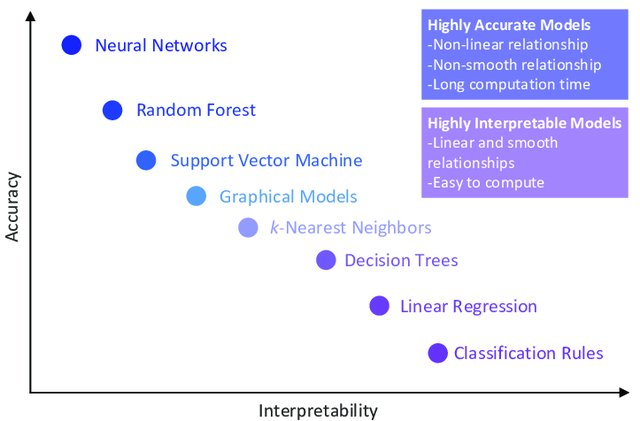
\includegraphics[scale=1.4]{images/interpretability_accuracy_tradeoff.jpg}
    \caption{The plot represented the trade-off between accuracy and intepretability of most common model \cite{morocho2019machine}.}
    \label{fig:trade-off}
\end{figure}
\subsection{Neural Network with Keras}
It is one of the deep learning algorithms which is based on the structure of the \gls{nn}, where nodes represent neurons.
Nodes are connected to each other through the layers. \\
In this way, every neuron of a layer is connected to neurons in the next layer.
The structure of my Neural Network is formed by 3 layers:
\begin{itemize}
    \item Input layer: Each node takes the initial data into the network and propagates information to the following layers;
    \item Output layer: It contains the result of the problem. 
    \item Hidden layer: It's actually responsible for the performance and complexity of neural networks. It's placed between the output and input layers;
\end{itemize}
During the training phase, in which the network "learns", independent variables are used as input and processed through weighted associations in which at each step the produced results are compared to the target output.\\ The difference computed between them is successively adjusted and updated following the learning rules. The achievement obtained is a result increasingly similar to the values assumed by the target variable.\\ 
For implementing it, I use Keras API from TensorFlow library \cite{tensorflow}.


\subsection{Machine Learning with Random Forest}
Random forests are used in regression problems, using a decision tree structure to make predictions. Decision trees answer sequential questions through the routes tracked by trees.\\
The algorithm consists in building a certain number of random decision trees from the bootstrap sample of the original data set (this phase is called bootstrap sampling). Then, the prediction of a certain sample is performed by following each decision tree. \\In a regression problem, the final decision will be an averaged value from the ones obtained by each tree (phase of aggregation).\\
To implement it, I used RandomForestRegressor class from sklearn library. 


\begin{figure}[H]
    \centering
    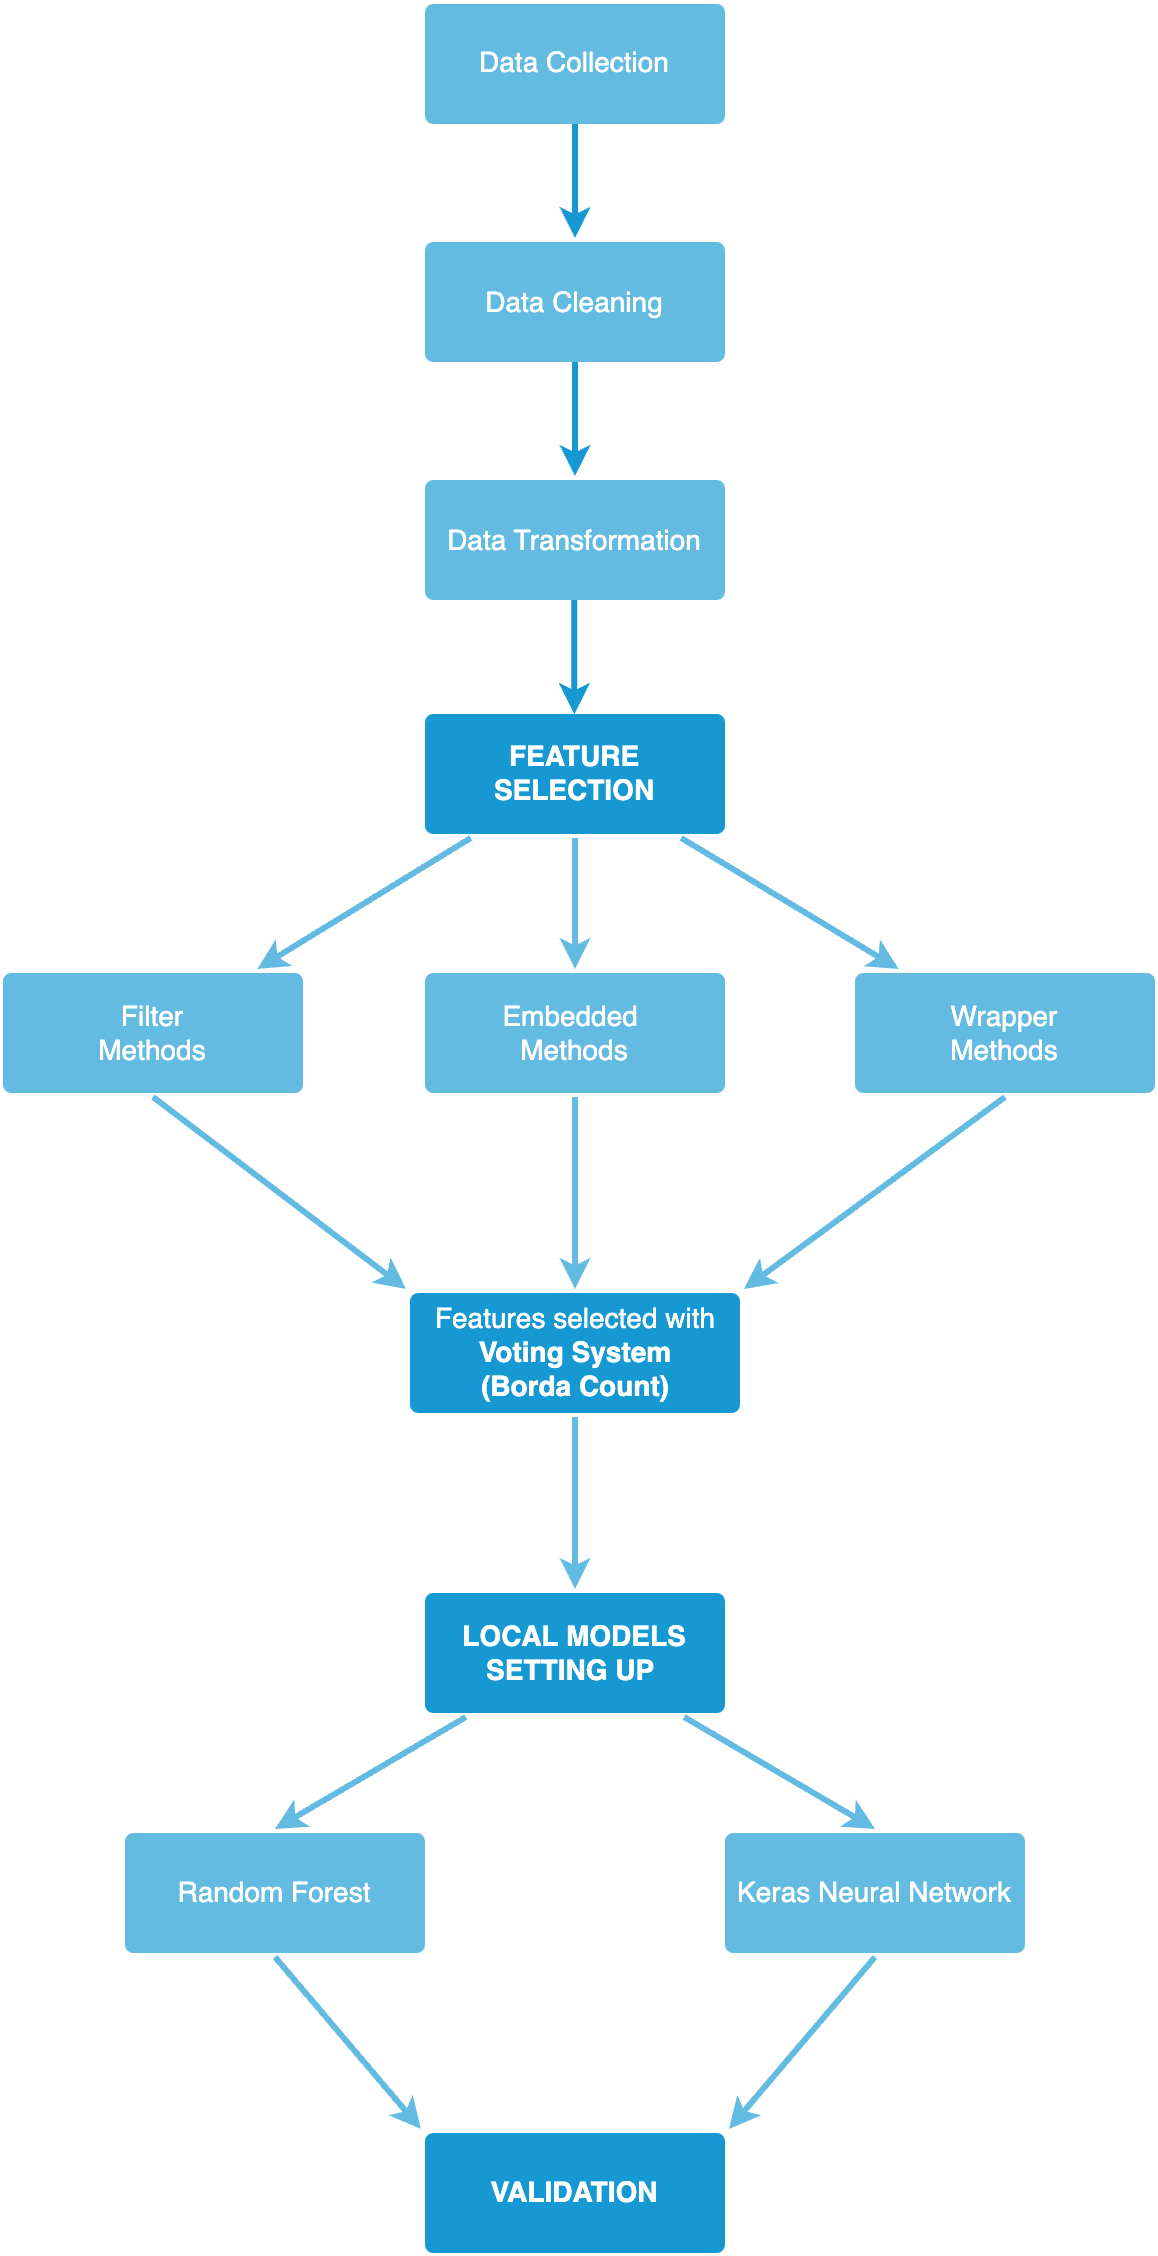
\includegraphics[scale=0.21]{images/overview.png}
    \caption{Overview of the steps made in my work.}
    \label{fig:overview}
\end{figure}

The diagram in figure \ref{fig:overview} gives a general explanation of the procedure taken in this thesis. It starts with the pre-processing of the data (collection, cleaning and transformation) and continues with the selection of the most meaningful variables (feature selection). \\
After that, ML models are implemented and trained with the covariates chosen in the previous step. \\
Finally, an evaluation of the error metrics based on the validation is performed.
\section{Notebook implemented}
For processing and analyzing data, I implemented tools collected in Python Notebooks, each one available in the D-DUST repository\footnote{\url{https://github.com/opengeolab/D-DUST/tree/thesis_MB}}.\newline

\subsection{Computation and view of feature selection results}
In order to manage its configuration and the results obtained, a notebook\footnote{\url{https://github.com/opengeolab/D-DUST/blob/thesis_MB/notebooks/fs_results.ipynb}} with a simple user interface using the ipywidgets package was developed.
In this interface there are 2 sections:
\begin{itemize}
\item Feature Selection scores: they are graphically shown using multiple barplots, one for each data set previously selected. Barplot are implemented with the use of Plotly library; 
\item Options: in this box it is possible to configure the feature selection input:
\begin{itemize}
\item target variable. in our case the usable variables are those coming from ARPA ground sensors;
\item apply (optional) low variance filter for discarding meaningless variable before FS;
\end{itemize}
and the output:
\begin{itemize}
\item choice of method for visualizing its scores;
\item results normalization (optional);
\item order of the scores by descending order or by labels;
\item scale of Y-axis (regular or logarithmic);
\end{itemize}
\end{itemize}
A pseudo-code of how the notebook works is attached in the next page.\pagebreak
\begin{verbatim}
for each configuration in configurations
    for each period in periods
        #Data acquisition
        grid = input(period)
        data_cleaning(grid)
        grid = quasi_zeroVar(X)
        X, Y = get_variables(grid, target_variable)
        #Feature selection phase
        results = compute_feature_selection(X, Y)
    results = borda_count_algorithm(results)
    #results are stored externally in .csv files
    export_tocsv(results) 
    #results exported will have the feature ordered with respect
    #the score obtained with Borda Count algorithm
\end{verbatim}
\begin{figure}[H]
    \centering
    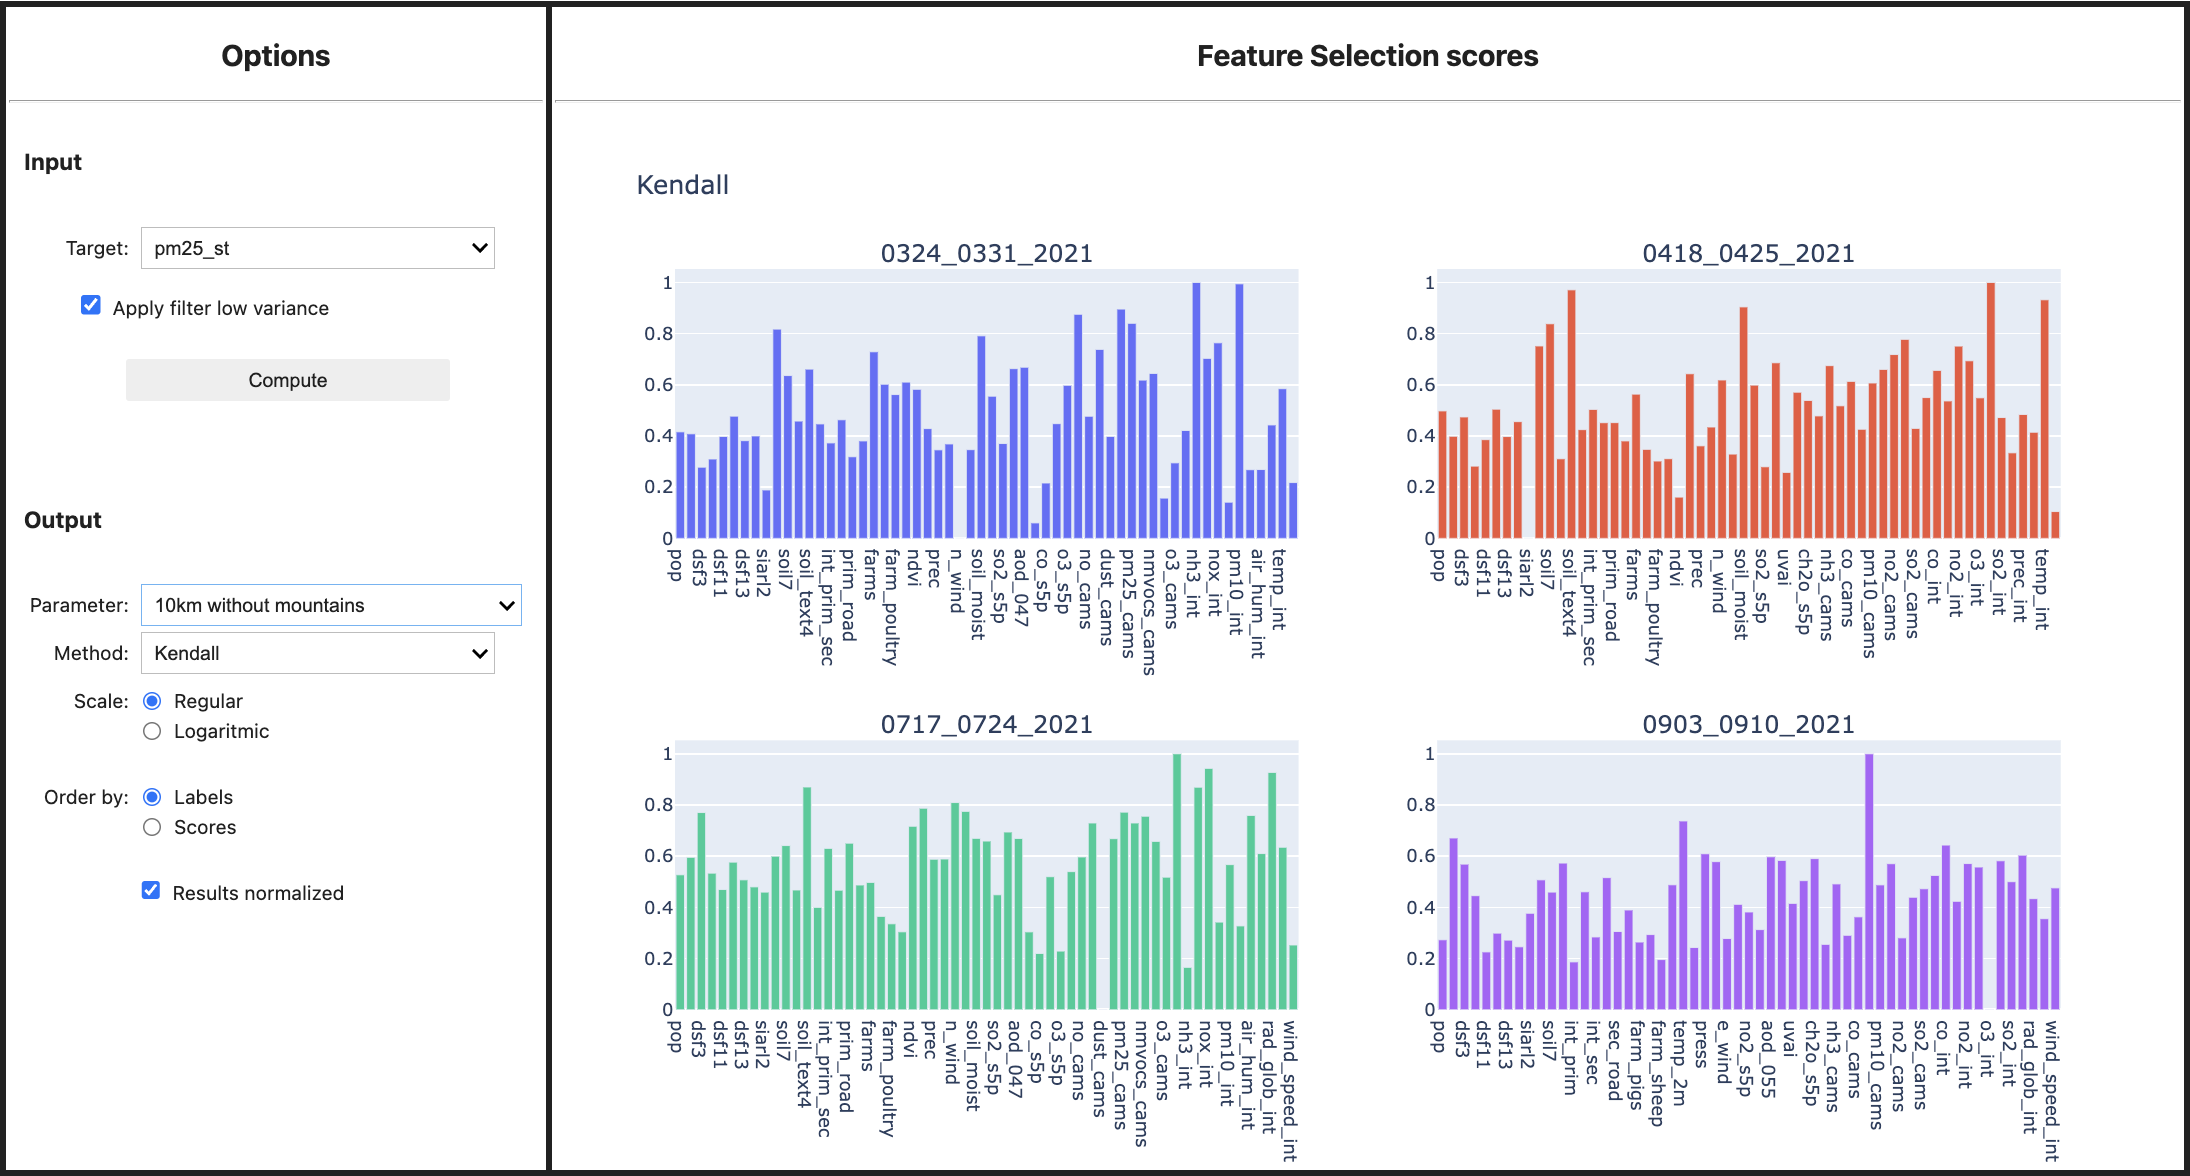
\includegraphics[scale=0.40]{images/notebook.png}
    \caption{Overview of the notebook implemented for FS procedure.In the notebook, there are also cells which aim to export FS results.}
    \label{fig:notebook}
\end{figure}
\pagebreak


\subsection{Computation and view of ML models results}
In order to build prediction model, I use two different notebooks for the evaluation of the Neural Network\footnote{\url{https://github.com/opengeolab/D-DUST/blob/thesis_MB/notebooks/Keras_prediction_model.ipynb}} and the Random Forest \footnote{\url{https://github.com/opengeolab/D-DUST/blob/thesis_MB/notebooks/RandomForest_prediction_model.ipynb}} models. 
It is possible to set these parameters before running the model:
\begin{itemize}
    \item NUMBER\_OF\_COVARIATES: it is the number of the n features with the highest Borda Count score taken as input for the model;
    \item TARGET: it represents the target variable to be predicted by the model;
\end{itemize}
\begin{verbatim}
for each configuration in configurations
    results = []
    for each period in periods
        #Data acquisition
        grid = input(period)
        grid = buffer_knn(grid)
        data_cleaning(grid)
        X, Y = get_variables(grid, TARGET)
        X = get_n_columns(NUMBER_OF_COVARIATES)
        #Modelling in which training and validation are performed using k-fold
        model = new()
        model.training(X, Y)
        res = model.validation(X, Y)
        results.append(res)
    
    #results are stored externally in .csv files
    export(avg(results1))
    export(avg(results2))
 
\end{verbatim}

Each of them imports the feature selected from the previous notebook and exports the accuracy evaluation of the k-fold cross-validation externally. \par
The results are subsequently opened and shown with
this other notebook\footnote{\url{https://github.com/opengeolab/D-DUST/blob/thesis_MB/notebooks/model.ipynb}} through the use of widgets (figure \ref{fig:view}), by simply  selecting the target variable, resolution and configuration desired.
\begin{figure}[H] 
    \centering
    \subfloat[Drop-down widgets.]{%
        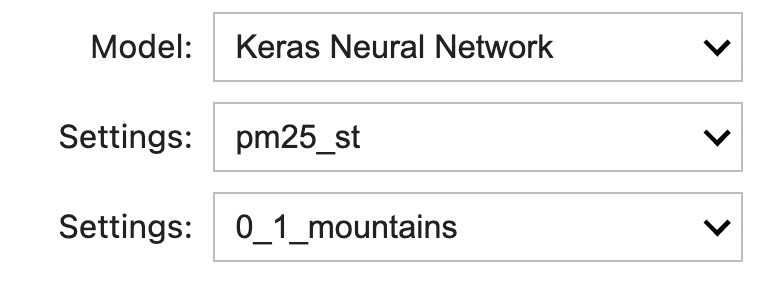
\includegraphics[width=0.5\textwidth]{images/dropdown.png}%
        %
        }%
    \hfill%
    \subfloat[Table with the results selected.]{%
        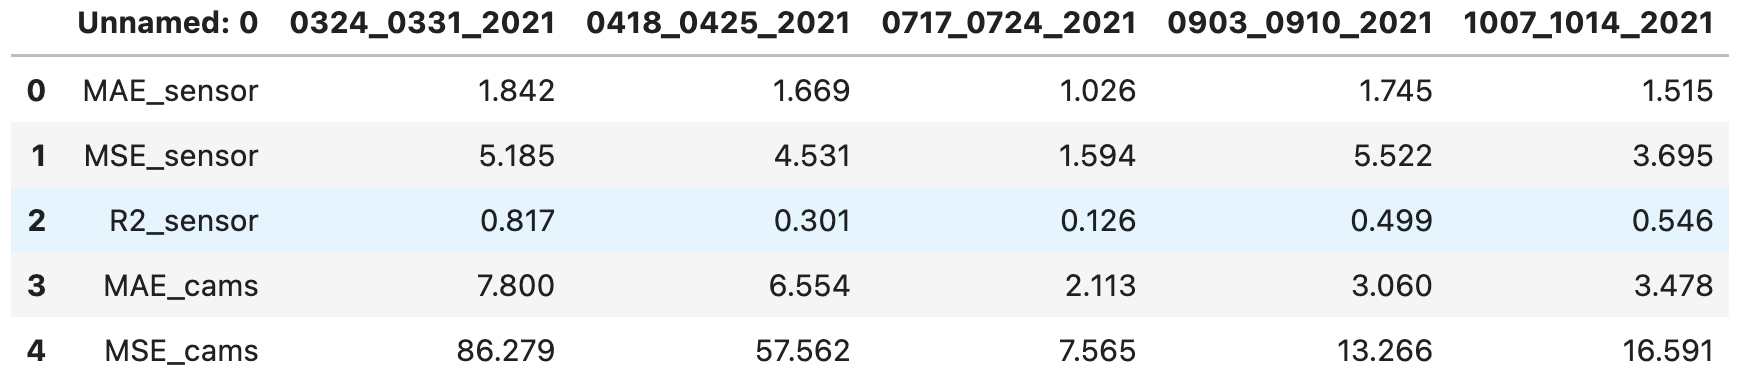
\includegraphics[width=0.5\textwidth]{images/table.png}%
        %
        }%
    \caption{In these images is illustrated how the results are viewed in the notebook (model.ipynb).}
    \label{fig:view}
\end{figure}

An overview of the order in which the different notebooks are used in my work thesis is illustrated in figure \ref{fig:notebooks}.
The first notebook used is fs\_results.ipynb which is used to preprocess the data and evaluate the FS results. \\
After that, the notebooks called Keras\_prediction\_model.ipynb and RandomForest\_prediction\_model.ipynb are used to implement ML models which are trained with the covariates chosen in the previous step. \\
Finally, the results of the error metrics based on the validation are provided by model.ipynb notebook. 
\par
In the next chapters, each step will be described in detail about the procedures adapted for the study case and the results obtained.
\begin{figure}[H]
    \centering
    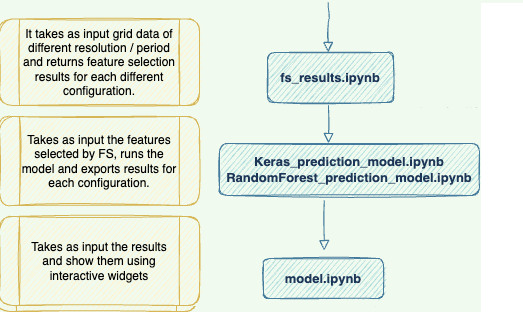
\includegraphics[scale=0.40]{images/overview _notebooks.png}
    \caption{Overview of the order in which the notebooks are used in my work.}
    \label{fig:notebooks}
\end{figure}